%%% Hlavní soubor. Zde se definují základní parametry a odkazuje se na ostatní části. %%%

%% Verze pro jednostranný tisk:
% Okraje: levý 40mm, pravý 25mm, horní a dolní 25mm
% (ale pozor, LaTeX si sám přidává 1in)
\documentclass[12pt,a4paper]{report}
\setlength\textwidth{145mm}
\setlength\textheight{247mm}
\setlength\oddsidemargin{15mm}
\setlength\evensidemargin{15mm}
\setlength\topmargin{0mm}
\setlength\headsep{0mm}
\setlength\headheight{0mm}
% \openright zařídí, aby následující text začínal na pravé straně knihy
\let\openright=\clearpage

%% Pokud tiskneme oboustranně:
% \documentclass[12pt,a4paper,twoside,openright]{report}
% \setlength\textwidth{145mm}
% \setlength\textheight{247mm}
% \setlength\oddsidemargin{14.2mm}
% \setlength\evensidemargin{0mm}
% \setlength\topmargin{0mm}
% \setlength\headsep{0mm}
% \setlength\headheight{0mm}
% \let\openright=\cleardoublepage

%% Vytváříme PDF/A-2u
\usepackage[a-2u]{pdfx}

%% Přepneme na českou sazbu a fonty Latin Modern
\usepackage[czech]{babel}
\usepackage{lmodern}
\usepackage[T1]{fontenc}
\usepackage{textcomp}

%% Použité kódování znaků: obvykle latin2, cp1250 nebo utf8:
\usepackage[utf8]{inputenc}

%%% Další užitečné balíčky (jsou součástí běžných distribucí LaTeXu)
\usepackage{amsmath}        % rozšíření pro sazbu matematiky
\usepackage{amsfonts}       % matematické fonty
\usepackage{amsthm}         % sazba vět, definic apod.
\usepackage{bbding}         % balíček s nejrůznějšími symboly
			    % (čtverečky, hvězdičky, tužtičky, nůžtičky, ...)
\usepackage{bm}             % tučné symboly (příkaz \bm)
\usepackage{graphicx}       % vkládání obrázků
\usepackage{fancyvrb}       % vylepšené prostředí pro strojové písmo
\usepackage{indentfirst}    % zavede odsazení 1. odstavce kapitoly
\usepackage{natbib}         % zajištuje možnost odkazovat na literaturu
			    % stylem AUTOR (ROK), resp. AUTOR [ČÍSLO]
\usepackage[nottoc]{tocbibind} % zajistí přidání seznamu literatury,
                            % obrázků a tabulek do obsahu
\usepackage{icomma}         % inteligetní čárka v matematickém módu
\usepackage{dcolumn}        % lepší zarovnání sloupců v tabulkách
\usepackage{booktabs}       % lepší vodorovné linky v tabulkách
\usepackage{paralist}       % lepší enumerate a itemize
\usepackage{colortbl}			%tabulka
\usepackage{algpseudocode} 		%kod
\usepackage[usenames]{xcolor}  % barevná sazba

%%% Údaje o práci

% Název práce v jazyce práce (přesně podle zadání)
\def\NazevPrace{Varianty Eberhardovy věty}

% Název práce v angličtině
\def\NazevPraceEN{Eberhard-Like Theorems}

% Jméno autora
\def\AutorPrace{Zuzana Šimečková}

% Rok odevzdání
\def\RokOdevzdani{2018}

% Název katedry nebo ústavu, kde byla práce oficiálně zadána
% (dle Organizační struktury MFF UK, případně plný název pracoviště mimo MFF)
\def\Katedra{Informatický ústav Univerzity Karlovy}
\def\KatedraEN{Computer Science Institute of~Charles University}

% Jedná se o katedru (department) nebo o ústav (institute)?
\def\TypPracoviste{Ústav}
\def\TypPracovisteEN{Institute}

% Vedoucí práce: Jméno a příjmení s~tituly
\def\Vedouci{doc. Mgr. Robert Šámal, Ph.D.}

% Pracoviště vedoucího (opět dle Organizační struktury MFF)
\def\KatedraVedouciho{Informatický ústav Univerzity Karlovy}
\def\KatedraVedoucihoEN{Computer Science Institute of~Charles University}

% Studijní program a obor
\def\StudijniProgram{Informatika}
\def\StudijniObor{IOI}

% Nepovinné poděkování (vedoucímu práce, konzultantovi, tomu, kdo
% zapůjčil software, literaturu apod.)
\def\Podekovani{%
Děkuji doc. Mgr. Robertu Šámalovi, Ph.D., vedoucímu práce, za~ochotu, trpělivost, odborné rady a~čas, které mi věnoval. Za~výběr tématu a~připomínky při~řešení i~sepisování práce.
}

% Abstrakt (doporučený rozsah cca 80-200 slov; nejedná se o zadání práce)
\def\Abstrakt{%
Pro konkrétní nakreslení rovinného grafu definujme posloupnost $(p_k)=(p_3,p_4,\dots)$ počtů k-hranných stěn -- $k$-úhelníků. Důsledkem Eulerova vzorce o~rovinných grafech pro kubické grafy splňuje $p$ vztah $\sum_{k \geq 3}{(6-k)p_k}=12$. Je celkem přirozené ptát se, jak vypadají $p$, pro která existuje odpovídající graf. Eberhard ukázal, že pokud $p$ splňuje výše uvedenou rovnost, pak existuje rovinný kubický graf, který odpovídá $p$ až na počet šestiúhelníků. DeVos a kol. dokázali obdobu věty, kde je povoleno k $p$ přidat pětiúhelníky a sedmiúhelníky. V této práci na jejich výsledky navazujeme, využijeme jejich důkazové strategie a díky navrženému programu najdeme stavební bloky, které autorům k zobecnění věty chyběly. Výsledkem práce je následující věta: pro každou dvojici $r,s \in \mathbb{N} $ splňující $ s<6<r<14, s,r$ nesoudělné, platí následující věta: pro každou posloupnost $p$ nezáporných celých čísel splňující $\sum_{k \geq 3}{(6-k)p_k}=12$ existuje nekonečně mnoho kubických rovinných grafů, které $p$ odpovídají až na $r$-úhelníky a $s$-úhelníky. 
}
\def\AbstraktEN{%
Define sequence $(p_k)=(p_3,p_4,\dots)$  as numbers of $k$-sized faces -- k-gons -- of an embedding of a planar graph. A corollary to Euler’s formula for planar graphs states that for cubic graphs  $\sum_{k \geq 3}{(6-k)p_k}=12$ holds. Naturally, this leads us to explore the nature of p for which a corresponding cubic planar graph exists. Eberhard proved that if $p$ satisfies the equality above then a cubic planar graph that corresponds to $p$ except for the number of hexagons, exists. DeVos et al. show similar theorem, but instead of hexagon, both pentagons and heptagons can be added. In this thesis, we follow up their result by using their proof strategy and designing a program to find graphs needed in such proof. We were able to prove that $ \forall r,s \in  \mathbb{N}$ where $ s<6<r<14$ and $r,s $ are coprime the following theorem holds: for each sequence of nonnegative integers satisfying  $\sum_{k \geq 3}{(6-k)p_k}=12$ there are infinitely many cubic planar graphs corresponding to $p$ except for the number of both $r$-gons and $s$-gons.
}

% 3 až 5 klíčových slov (doporučeno), každé uzavřeno ve složených závorkách
\def\KlicovaSlova{%
{kubické grafy} {rovinné grafy} {Eberhardova věta} {kreslení grafů} 
}
\def\KlicovaSlovaEN{%
{cubic graphs} {planar graphs} {Eberhard's theorem} {graph drawing}
}

%% Balíček hyperref, kterým jdou vyrábět klikací odkazy v PDF,
%% ale hlavně ho používáme k uložení metadat do PDF (včetně obsahu).
%% Většinu nastavítek přednastaví balíček pdfx.
\hypersetup{unicode}
\hypersetup{breaklinks=true}

%% Definice různých užitečných maker (viz popis uvnitř souboru)
%%% Tento soubor obsahuje definice různých užitečných maker a prostředí %%%
%%% Další makra připisujte sem, ať nepřekáží v ostatních souborech.     %%%

%%% Drobné úpravy stylu

% Tato makra přesvědčují mírně ošklivým trikem LaTeX, aby hlavičky kapitol
% sázel příčetněji a nevynechával nad nimi spoustu místa. Směle ignorujte.
\makeatletter
\def\@makechapterhead#1{
  {\parindent \z@ \raggedright \normalfont
   \Huge\bfseries \thechapter. #1
   \par\nobreak
   \vskip 20\p@
}}
\def\@makeschapterhead#1{
  {\parindent \z@ \raggedright \normalfont
   \Huge\bfseries #1
   \par\nobreak
   \vskip 20\p@
}}
\makeatother

% Toto makro definuje kapitolu, která není očíslovaná, ale je uvedena v obsahu.
\def\chapwithtoc#1{
\chapter*{#1}
\addcontentsline{toc}{chapter}{#1}
}

% Trochu volnější nastavení dělení slov, než je default.
\lefthyphenmin=2
\righthyphenmin=2

% Zapne černé "slimáky" na koncích řádků, které přetekly, abychom si
% jich lépe všimli.
%\overfullrule=1mm

%%% Makra pro definice, věty, tvrzení, příklady, ... (vyžaduje baliček amsthm)

\theoremstyle{plain}
\newtheorem{veta}{Věta}
\newtheorem{lemma}[veta]{Lemma}
\newtheorem{tvrz}[veta]{Pozorování}
\newtheorem{hypot}[veta]{Hypotéza}

\theoremstyle{plain}
\newtheorem{definice}{Definice}

\theoremstyle{remark}
\newtheorem*{dusl}{Důsledek}
\newtheorem*{pozn}{Poznámka}
\newtheorem*{prikl}{Příklad}

%%% Prostředí pro důkazy

\newenvironment{dukaz}{
  \par\medskip\noindent
  \textit{Důkaz}.
}{
\newline
\rightline{$\square$}  % nebo \SquareCastShadowBottomRight z balíčku bbding
}

%%% Prostředí pro sazbu kódu, případně vstupu/výstupu počítačových
%%% programů. (Vyžaduje balíček fancyvrb -- fancy verbatim.)

\DefineVerbatimEnvironment{code}{Verbatim}{fontsize=\small, frame=single}

%%% Prostor reálných, resp. přirozených čísel
\newcommand{\R}{\mathbb{R}}
\newcommand{\N}{\mathbb{N}}

%%% Užitečné operátory pro statistiku a pravděpodobnost
\DeclareMathOperator{\pr}{\textsf{P}}
\DeclareMathOperator{\E}{\textsf{E}\,}
\DeclareMathOperator{\var}{\textrm{var}}
\DeclareMathOperator{\sd}{\textrm{sd}}

%%% Příkaz pro transpozici vektoru/matice
\newcommand{\T}[1]{#1^\top}

%%% Vychytávky pro matematiku
\newcommand{\goto}{\rightarrow}
\newcommand{\gotop}{\stackrel{P}{\longrightarrow}}
\newcommand{\maon}[1]{o(n^{#1})}
\newcommand{\abs}[1]{\left|{#1}\right|}
\newcommand{\dint}{\int_0^\tau\!\!\int_0^\tau}
\newcommand{\isqr}[1]{\frac{1}{\sqrt{#1}}}

%%% Vychytávky pro tabulky
\newcommand{\pulrad}[1]{\raisebox{1.5ex}[0pt]{#1}}
\newcommand{\mc}[1]{\multicolumn{1}{c}{#1}}


%% Titulní strana a různé povinné informační strany
\begin{document}
%%% Titulní strana práce a další povinné informační strany

%%% Titulní strana práce

\pagestyle{empty}
\hypersetup{pageanchor=false}

\begin{center}

\centerline{\mbox{
\includegraphics[width=166mm]{../img/logo-cs.pdf}}}

\vspace{-8mm}
\vfill

{\bf\Large BAKALÁŘSKÁ PRÁCE}

\vfill

{\LARGE\AutorPrace}

\vspace{15mm}

{\LARGE\bfseries\NazevPrace}

\vfill

\Katedra

\vfill

\begin{tabular}{rl}

Vedoucí bakalářské práce: & \Vedouci \\
\noalign{\vspace{2mm}}
Studijní program: & \StudijniProgram \\
\noalign{\vspace{2mm}}
Studijní obor: & \StudijniObor \\
\end{tabular}

\vfill

% Zde doplňte rok
Praha \RokOdevzdani

\end{center}

\newpage

%%% Následuje vevázaný list -- kopie podepsaného "Zadání bakalářské práce".
%%% Toto zadání NENÍ součástí elektronické verze práce, nescanovat.

%%% Strana s čestným prohlášením k bakalářské práci

\openright
\hypersetup{pageanchor=true}
\pagestyle{plain}
\pagenumbering{roman}
\vglue 0pt plus 1fill

\noindent
Prohlašuji, že jsem tuto bakalářskou práci vypracovala samostatně a výhradně
s~použitím citovaných pramenů, literatury a dalších odborných zdrojů.

\medskip\noindent
Beru na~vědomí, že se na moji práci vztahují práva a povinnosti vyplývající
ze zákona č. 121/2000 Sb., autorského zákona v~platném znění, zejména skutečnost,
že Univerzita Karlova má právo na~uzavření licenční smlouvy o~užití této
práce jako školního díla podle §60 odst. 1 autorského zákona.

\vspace{10mm}

\hbox{\hbox to 0.5\hsize{%
V ........ dne ............
\hss}\hbox to 0.5\hsize{%
Podpis autora
\hss}}

\vspace{20mm}
\newpage

%%% Poděkování

\openright

\noindent
\Podekovani

\newpage

%%% Povinná informační strana bakalářské práce

\openright

\vbox to 0.5\vsize{
\setlength\parindent{0mm}
\setlength\parskip{5mm}

Název práce:
\NazevPrace

Autor:
\AutorPrace

\TypPracoviste:
\Katedra

Vedoucí bakalářské práce:
\Vedouci, \KatedraVedouciho

Abstrakt:
\Abstrakt

Klíčová slova:
\KlicovaSlova

\vss}\nobreak\vbox to 0.49\vsize{
\setlength\parindent{0mm}
\setlength\parskip{5mm}

Title:
\NazevPraceEN

Author:
\AutorPrace

\TypPracovisteEN:
\KatedraEN

Supervisor:
\Vedouci, \KatedraVedoucihoEN

Abstract:
\AbstraktEN

Keywords:
\KlicovaSlovaEN

\vss}

\newpage

\openright
\pagestyle{plain}
\pagenumbering{arabic}
\setcounter{page}{1}


%%% Strana s automaticky generovaným obsahem bakalářské práce

\tableofcontents

%%% Jednotlivé kapitoly práce jsou pro přehlednost uloženy v samostatných souborech
\chapter*{Úvod}
\addcontentsline{toc}{chapter}{Úvod}

Následuje několik ukázkových kapitol, které doporučují, jak by se
měla bakalářská práce sázet. Primárně popisují použití \TeX{}ové
šablony, ale obecné rady poslouží dobře i~uživatelům jiných
systémů.

%%% Fiktivní kapitola s ukázkami sazby

\chapter{Pojmy a definice}

Pokud čtenář není seznámen se základy teorie grafů, doporučujeme začít třeba knihou Kapitoly z diskrétní matematiky \cite{Matousek}. Před zadefinováním základní terminologie pro~tuto práci dokažme nejprve, jak z Eulerova vzorce získáme~\eqref{eq01:neccCond}. Doplňmě navíc, že -- pokud není řečeno jinak -- uvažujeme pouze souvislé grafy a to ve všech větách i důkazech.

\begin{dukaz}
Pro každý kubický graf $G = (V,E)$ platí $3 |V| = 2 |E|$. Obecně platí, že počet stěn $s$ můžeme přepsat následovně $s = \sum_{k \geq 3}{p_k}$ a pro rovinné grafy platí i~$ \sum_{k \geq 3}{k \cdot p_k}= 2|E|$, protože pokud pro každou stěnu započteme každou její hranu, získáme právě $2|E|$. Úpravou a dosazením do vzorce získáme požadovaný výraz: 
\begin{align*}
|V|-|E|+|S|=2 \\ -\frac{1}{3} |E| + s = 2 \\
-\frac{1}{6} \sum_{k \geq 3}{k \cdot p_k} + \sum_{k \geq 3}{p_k} = 2 \\ 
\sum_{k \geq 3}{(6-k)p_k}=12
\end{align*}
\end{dukaz}

Zaveďme nyní základní pojmy. Stěně rovinného grafu, která se skládá z $k$ hran, budeme říkat jednoduše \textbf{$\boldsymbol{k}$-úhelník}. Pokud máme posloupnost $(p_k) = (p_3,p_4,\dots)$, která bude představovat počty k-úhelníků v grafu, definujme $\boldsymbol{P} = \lbrace k \mid p_k \neq 0 \rbrace$ jako její \textbf{množinu stěn}.

Klasifikujme posloupnosti $(p_k) = (p_3,p_4,\dots)$ podle jejich vlastností.

\begin{definice}[Neutrální posloupnost]\label{def01:neutralni}
Posloupnost $(p_k) = (p_3,p_4,\dots)$ nezáporných celých čísel je neutrální, pokud $\sum_{k \geq 3}{(6-k)p_k}=0$.
\end{definice}

\begin{definice}[Přípustná posloupnost]\label{def01:pripustna}
Posloupnost $(p_k) = (p_3,p_4,\dots)$ nezáporných celých čísel je přípustná, pokud $\sum_{k \geq 3}{(6-k)p_k}=6$.
\end{definice}

\begin{definice}[Realizovatelná posloupnost]\label{def01:realizovatelna}
Posloupnost $(p_k) = (p_3,p_4,\dots)$ nezáporných celých čísel je realizovatelná, pokud existuje konečný rovinný kubický graf, který má právě $p_k$ $k$-úhelníků.
\end{definice}

Všimněme si, že původní Eberhardova věta, a i mnoho jejích variant, byla formulována pro 3-souvislé grafy, tedy přesněji pro jednoduché konvexní 3-polytopy. Bijekci mezi těmito dvěma strukturami dokázal až o~několik desítek let později Steinitz \cite{Steinitz}. 

Pro ujištění pojmů uveďme následující jednoduché vlastnosti neutrálních, přípustných a realizovatelných posloupností, které využijeme později.
\begin{tvrz}
Pro každou neutrální (či přípustnou nebo realizovatelnou) posloupnost $p=(p_3,p_4,\dots)$ existuje $h \in \mathbb{N}$, že $ \forall k \in \mathbb{N}, k>h $ platí $ p_k=0$.
\end{tvrz}

\begin{dukaz}
Neutrální posloupnost $p$ splňuje $\sum_{k \geq 3}{(6-k)p_k}=0$, což můžeme upravit na $\sum_{3 \leq k \leq 5}{(6-k)p_k}=\sum_{k \geq 5}{(k-6)p_k}$. Všechny sčítance na obou stranách výrazu jsou kladné. Hodnota levého součtu tří sčítanců je konečná. Pravý součet má tedy také konečnou hodnotu a navíc mají všechny jeho nenulové sčítance hodnotu alespoň 1. Nenulových hodnot v posloupnosti je tedy pouze konečně. 
\end{dukaz}

\begin{tvrz}\label{veta:posloupnosti}
\begin{description}
\item[] Pro každou $q$ neutrální posloupnost $\exists a,b \in Q : a <6 \wedge b>6$.
\item[] Součet dvou neutrálních posloupností je neutrální posloupnost. Součet neutrální a přípustné posloupnosti je přípustná posloupnost.
\item[] Pro každou přípustnou posloupnost $(p_k) = (p_3,p_4,\dots)$ existuje neutrální posloupnost $q$, že $p+qn$ je realizovatelná pro nějaké $n \in \mathbb{N}$.
\end{description}
\end{tvrz}

\begin{dukaz}
Pro ukázání první vlastnosti postačí, když si uvědomíme, že chceme $\sum_{k \geq 3}{(6-k)p_k} = 0$, kde pro $k < 6$ je sčítaný člen kladný, zato pro $k>6$ je sčítaný člen záporný. Druhá vlastnost plyne z definice a distributivity násobení. Třetí tvrzení pro je slabší verze Věty \ref{veta:Eberhard}.
\end{dukaz}
K poslední vlastnosti se nabízí otázka, jak lze $q$ omezit, aby pořád $p+qn$ byla realizovatelná. Eberhard ukázal, že stačí  $q = (0,0,0,q_6=1,0,\dots)$, tedy přidat šestiúhelníky. DeVos a kol. ukázal že i omezení na  $q = (0,0,1,0,1,0,\dots)$ funguje. V této práci ukážeme, že posloupností s pouze dvěma nenulovými hodnotami, které v tomto směru vyhovují, existuje výrazně víc.





\chapter{Strategie důkazu}

Představme hypotézu, kterou se snažíme ověřit.
\begin{hypot}\label{veta02:hypoteza}
Mějme přípustnou posloupnost $p=(p_k | 3 \leq k \neq 6)$ a neutrální posloupnost $q=(q_k \mid 3 \leq k \neq 6)$, pak existuje takové přirozené $n$, že $p+nq$ je realizovatelná.
\end{hypot}


V článku \cite{Samal09} autoři naznačují strategii důkazu, za předpokladu, že existují nějaké pomocné grafy. V další kapitole představíme způsob, jak takové grafy hledat. Teď se zaměříme na důkaz samotný, respektive nejprve představíme graf, který v důkazu pomáhal již Eberhardovi.

\section{Triarky a operace s nimi}

\begin{definice}[Triark]\label{def02:1}
Triark je takový rovinný graf $T$, že vrcholy jeho vnější stěny tvoří cyklus $C$, každý vnitřní vrchol (tj. vrcholy $T-C$) má v $T$ stupeň právě 3 a v $C$ jsou tři navzájem různé vrcholy $x$, $y$, $z$ stupně 2 -- \textbf{rohy}, že vrcholy každé ze tří cest v C, které vzniknou odstraněním rohů z C, mají střídavě stupeň 2 a 3, počínaje i konče stupněm 2.
\end{definice}

\textbf{Strana} triarku je každá z výše zmíněných cest v C, ke které na oba konce připojíme i příslušný roh. \textbf{Délka strany} triarku odpovídá počtu jejích vnitřních vrcholů stupně 2 v T. O triarku se stranami délky $a$, $b$, $c$ mluvíme jako o \textbf{($\boldsymbol{a}$, $\boldsymbol{b}$, $\boldsymbol{c}$)-triarku}. Poznamenejme, že na pořadí stran v názvu nezáleží (odpovídají rotacím a zrcadlení). Později využijeme ještě dalšího značení. \textbf{$\boldsymbol{M}$-triark} má vnitřní strany pouze velikostí z množiny $M$. \textbf{($\boldsymbol{a}$, $\boldsymbol{b}$, $\boldsymbol{c}$)$\boldsymbol{M}$-triark} je zároveň ($a$, $b$, $c$)-triark a $M$-triark. Tato značení využíváme i pro další typy grafů a jejich význam je analogický. U triarku přejímáme některé termíny používané pro trojúhelníky a jejich význam bude vždy intuitivní.

\begin{figure}[h!]\centering
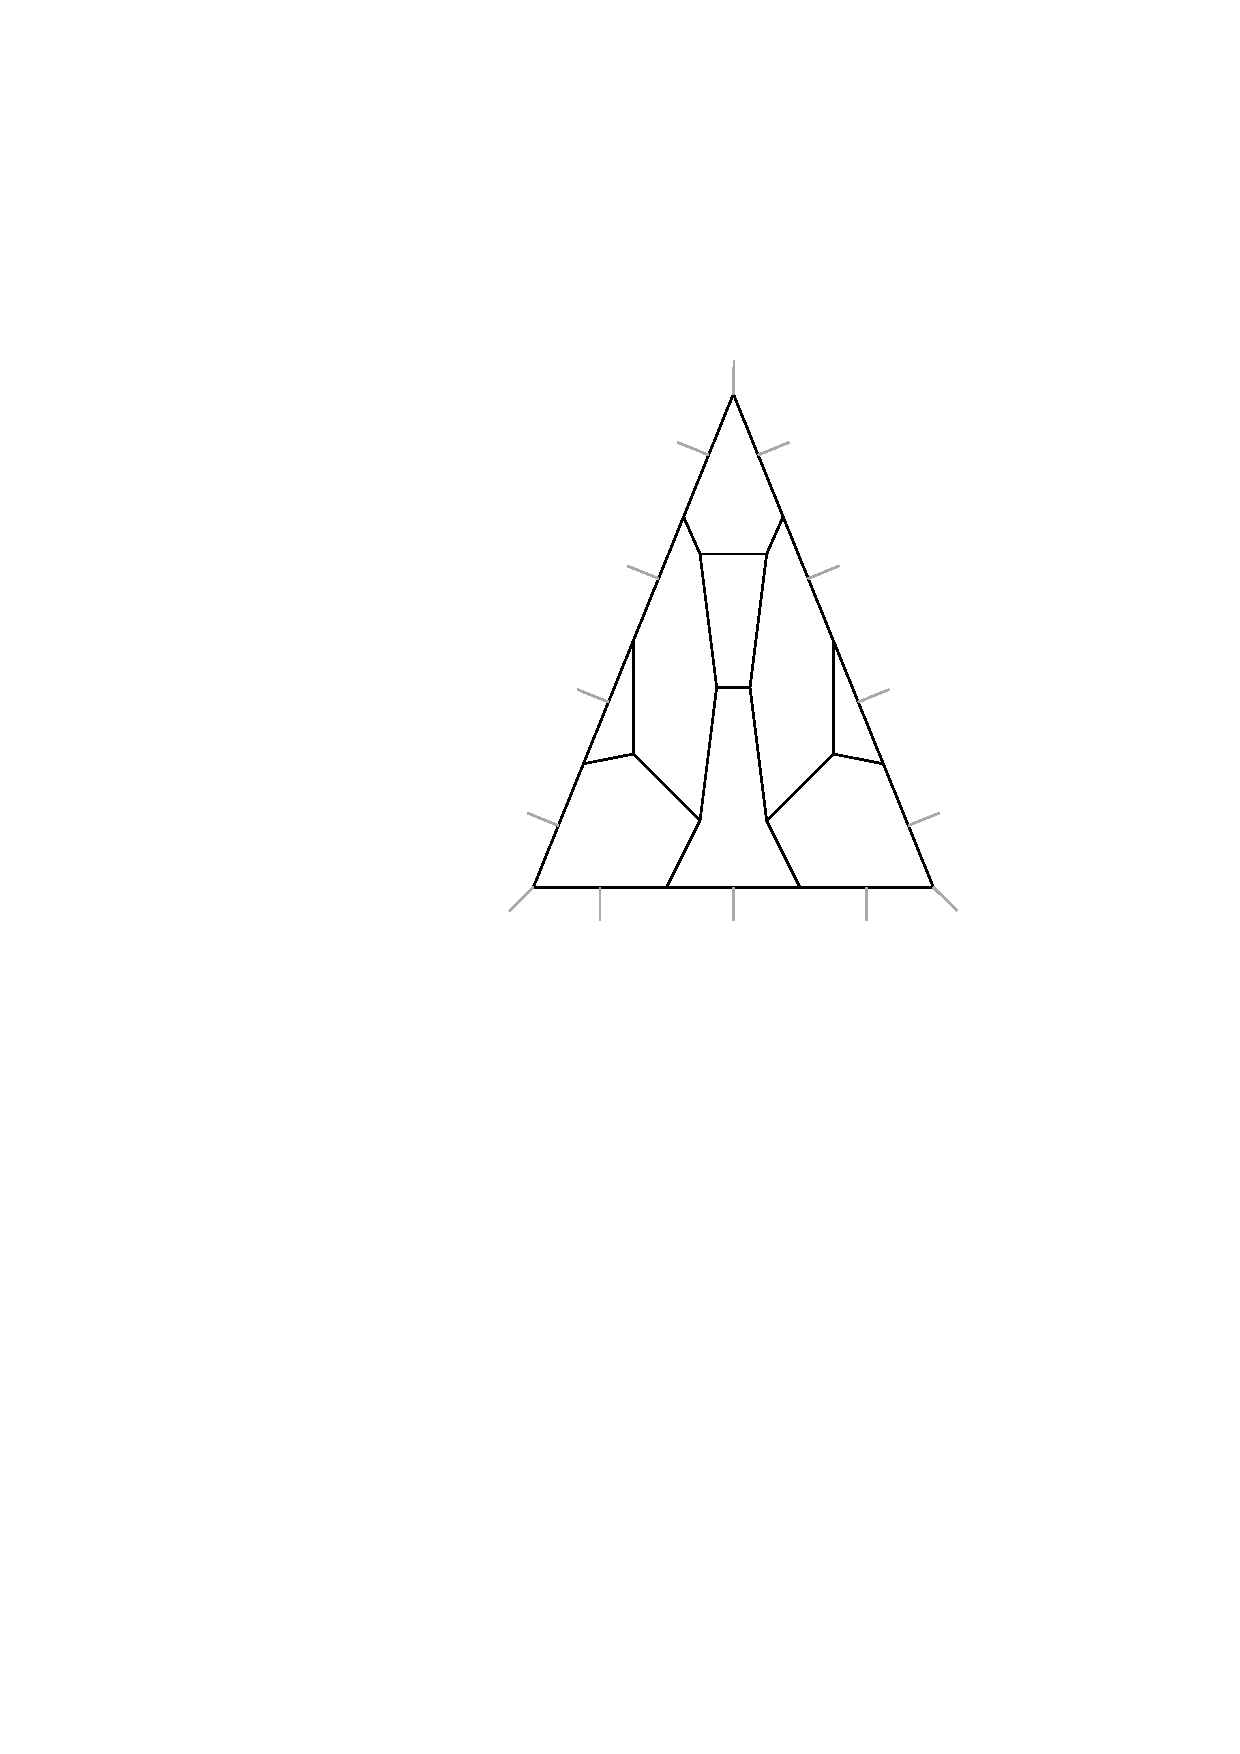
\includegraphics[height=60mm]{../img/triarc}
\caption{(4,4,3)$ \lbrace 4,7\rbrace $-triark.}
\label{obr03:triark}
\end{figure}

Zmiňme velmi užitečnou vlastnost triarků: pokud máme dva triarky, oba mající stranu stejné délky, můžeme je za tuto stranu slepit jako na Obrázku \ref{obr21:T-P} a získáme opět graf, jehož vnitřní vrcholy mají stupeň 3. (Při slepovaní se ztotožní vždy vrchol stupně 2 s vrcholem stupně 3.) Pokud slepíme triarky tak, že protější strany výsledného grafu budou stejně dlouhé (tedy speciálně při slepení dvou stejný triarků), budeme podle jeho tvaru mluvit o \textbf{rovnoběžníku}. Rovnoběžníky jdou navíc slepovat podobně jako triarky a můžeme tím každý již existující rovnoběžník zvětšit na libovolný rozměr, který je násobkem jeho původních rozměrů.


\begin{figure}[h!]\centering
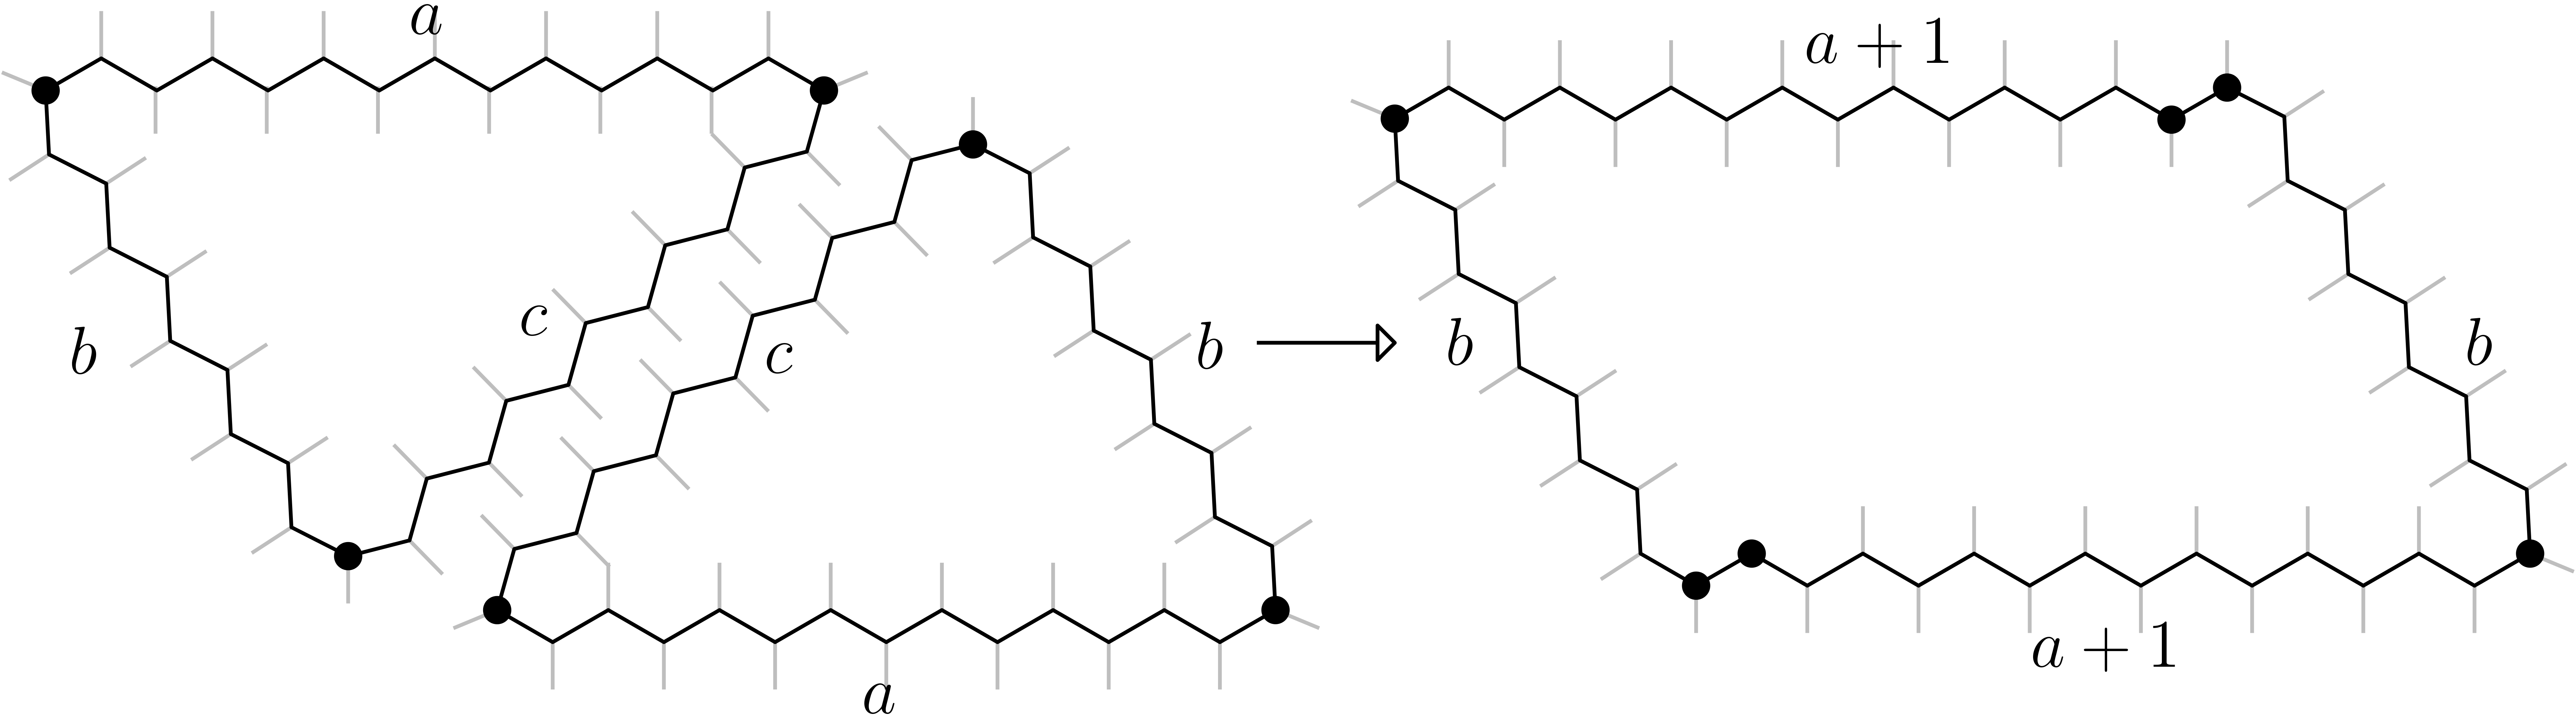
\includegraphics[width=\textwidth]{../img/T-P}
\caption{Spojení dvou triarků za vzniku rovnoběžníku.}
\label{obr21:T-P}
\end{figure}

Mohli bychom ale chtít spojovat triarky tak, aby výsledkem byl opět triark. Mějme ($a_1$, $b_1$, $c_1$)-triark a ($a_2$, $b_2$, $c_2$)-triark a vhodný rovnoběžník. Slepením, jako na Obrázku \ref{obr22:T-T}, vznikne ($a_1+a_2$, $b_1+b_2$, $c_1+c_2$)-triark. 

\begin{figure}[h!]\centering
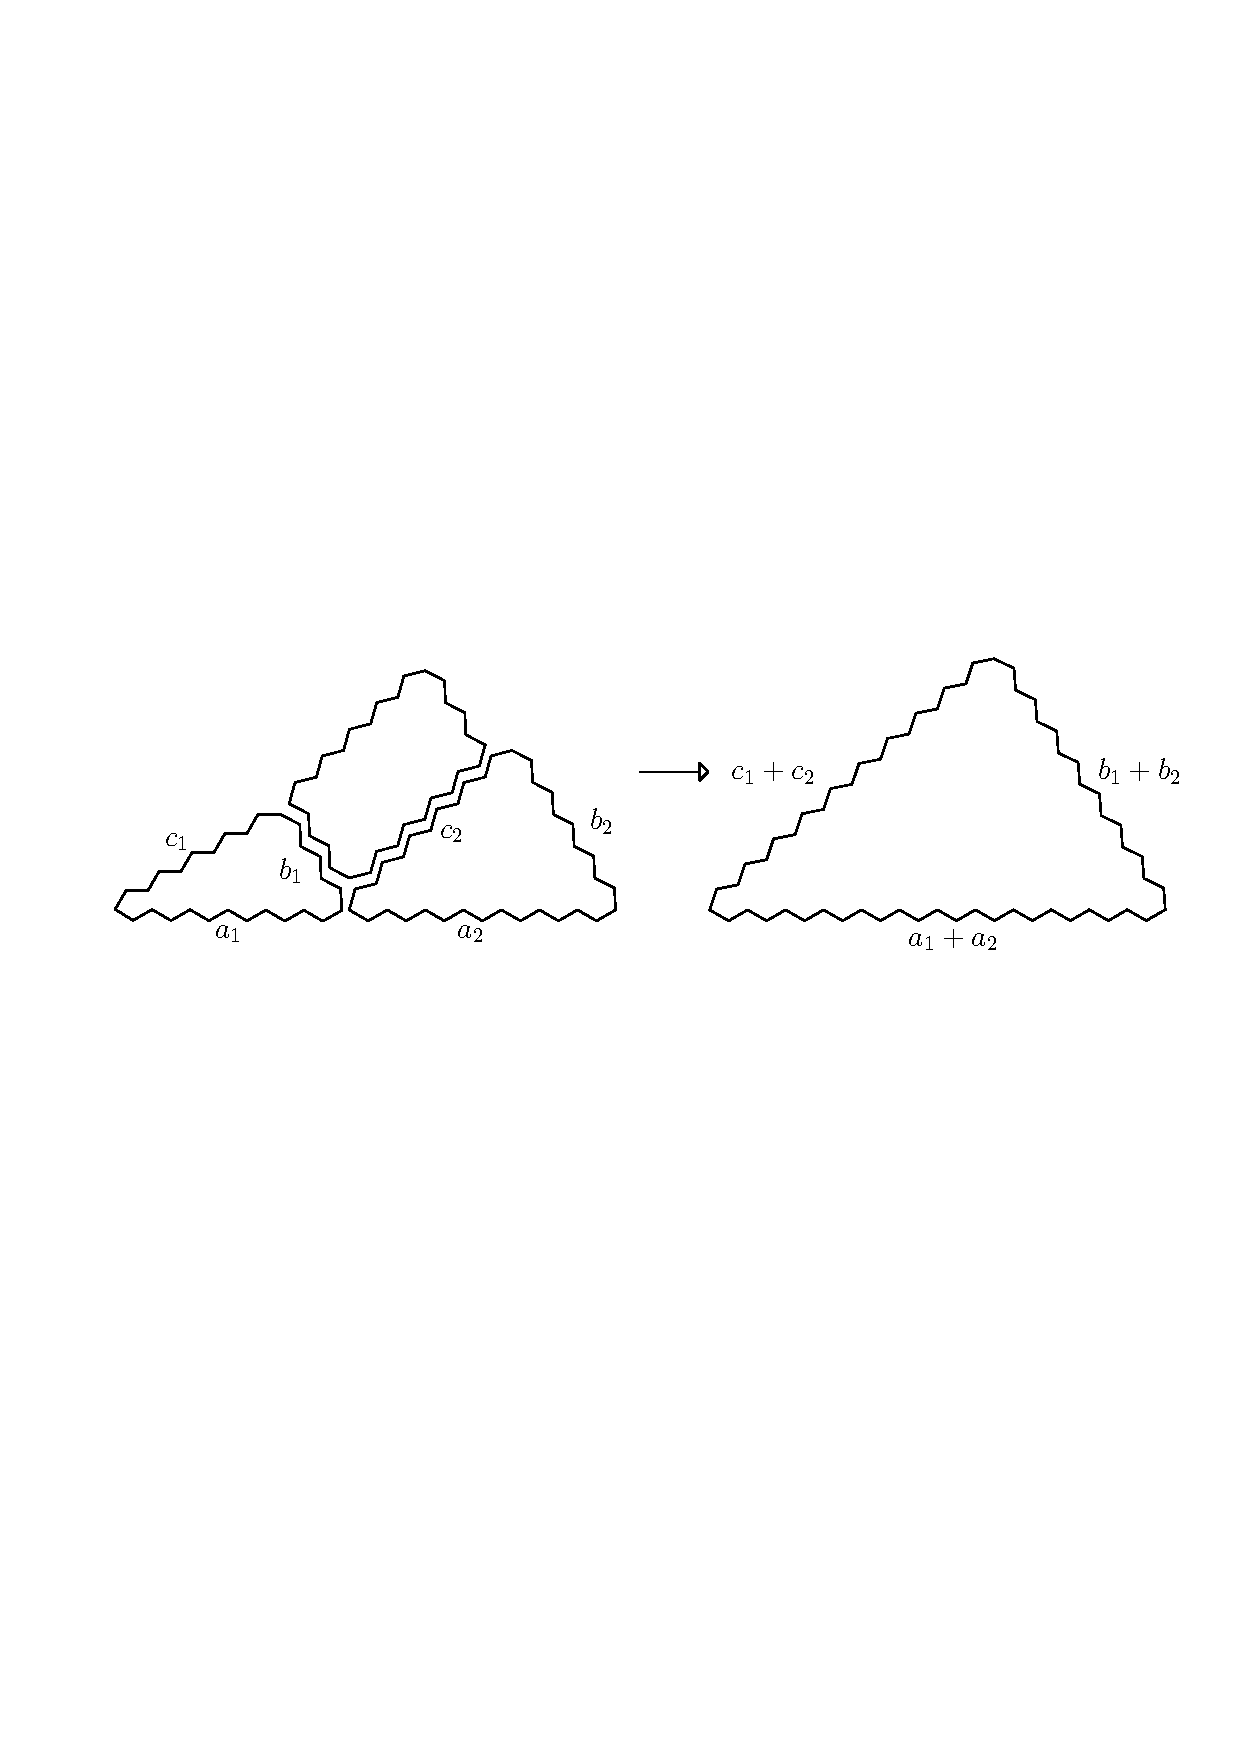
\includegraphics[width=\textwidth]{../img/T-T}
\caption{Spojení triarků spolu s rovnoběžníkem za vzniku triarku.}
\label{obr22:T-T}
\end{figure}

A závěrem budeme chtít spojit dva triarky tak, aby výsledkem byl kubický graf (tedy aby nevznikly žádné nové stěny s vrcholy stupně dva). Graf, který má tuto funkci označíme za \textbf{prstenec}. Pro lepší představu si prstenec představujme jako plášť trojbokého hranolu, triarky jako dolní a boční podstavu. Na všech podstavných hranách dojde ke splynutí vrcholů triarků s vrcholy prstence a vznikne graf nakreslitelný na hranol (tedy tedy i na sféru), takže výsledkem je rovinný graf. Zadefinujme prstenec formálně. Prstenec je souvislý kubický rovinný graf, ve kterém můžeme vyznačit dva disjunktní cykly tak, že stupně vrcholů každého cyklu jsou opačné než stupně příslušných triarků, které chceme spojit. Kde opačné znamená záměna dvoj- a tří- vaznosti vrcholů. Pro případné dokreslení můžeme použít Obrázek \ref{obr03:konstrukceiv}, na kterém je speciální druh prstence. 

%\begin{figure}[h!]\centering
%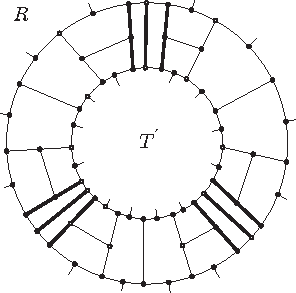
\includegraphics[height=40mm]{../img/T-G}
%\caption{Spojení triarků prstencem za vzniku kubického grafu.}
%\label{obr23:T-G}
%\end{figure}


\section{Důkaz za předpokladu existence pomocných grafů}
Převeďme hypotézu ve větu.

\begin{veta}\label{veta02:2}
Mějme přípustnou posloupnost $p=(p_k | 3 \leq k \neq 6)$ a neutrální posloupnost $q=(q_k \mid 3 \leq k \neq 6)$ a následující grafy pro nějaké přirozené k:
\begin{description}
\item[(i)] ($k$, $k$, $k$)$Q$-triark;
\item[(ii)] ($k$, $k$, $k-1$)$Q$-triark;
\item[(iii)] $\forall p_l \neq 0$ rovnoramenný $Q\cup \lbrace l \rbrace$-triark, délky jehož stejných stran jsou dělitelné $k$ a který obsahuje právě jednu stěnu velikosti $l$, této stěně říkejme \textbf{jádro} triarku;
\item[(iv)] $\forall t \in \mathbb{N}, t>1$ $Q$-prstenec, který dokáže spojit dva ($t$, $t$, $t$)-triarky.
\end{description} 

Pak existuje takové přirozené $n$, že $p+nq$ je realizovatelná.
\end{veta}


Myšlenka důkazu pak není příliš složitá: každou stěnu ze zadané posloupnosti $p$ zabalíme do triarku (iii), připravíme si pomocné lepicí a zkrášlující prvky (ii), díky kterým získáme jediný velký rovnostranný triark. K němu zkonstruujeme ještě jeden se stejně dlouhými stranami (i) a pomocným prstencem je spojíme v kýžený graf (iv). Všechny tyto pomocné objekty jsou totiž rovinné a (kromě jader) jen ze stěn, které jsou v zadané neutrální posloupnosti. Lepicí operace zachovávají kubičnost uvnitř grafu a prstenec pak spojí dva triarky v hledaný kubický graf.
\begin{dukaz}
Nejprve slepíme dva ($k$, $k$, $k-1$)-triarky za stěnu délky $k$ a získáme rovnoběžník se všemi stranami délky $k$. A díky slepování můžeme získat i libovolný rovnoběžník o rozměrech $mk$, $lk$ pro $m$, $l$ přirozená. Poté postupně spojujeme jednotlivé jádrové triarky za pomoci příslušného lichoběžníku, dokud nezískáme jediný triark, který obsahuje všechny stěny z $P$.

Zkusme vzniklý triark upravit na rovnostranný. Při slepování triarků se velikosti výsledných stran rovnají součtům původním. Pokud tedy slepujeme s ($k$, $k$, $k-1$)-triarkem, zmenšíme vždy tu stěnu, na kterou připadne rozměr $k-1$, vůči ostatním. Takže pokud budeme opakovat lepení výsledného triarku, v každém kroku se součet rozdílů mezi stranami zmenší a tedy nutně získáme rovnostranný triark. Modifikujme ho stejnou operací, aby zůstal rovnostranný, ale navíc délka jeho stran byla násobkem $k$ a označme výsledný triark $T_1$.

Slepováním ($k$,$k$,$k$)-triarků z (i) spolu s ($k$, $k$) rovnoběžníky získáme druhý triark $T_2$ o stejném rozměru jako $T_1$. Kdybychom celý problém řešili na toru, stačilo by $T_1$ a $T_2$ spojit do rovnoběžníku a sjednotit odpovídající strany. Na kouli místo toho použijeme prstenec z (iv). Tím získáme graf, který je kubický, rovinný a obsahuje požadované stěny. 
\end{dukaz}

Všimněme si, že větu jde jednoduše zesílit: nejen že za splnění předpokladů existuje nějaké $n \in \mathbb{N}$, pro které je $p+nq$ realizovatelná; existuje jich libovolně mnoho. V důkazu stačí před spojením $T_1$ a $T_2$ prstencem nejprve oba triarky slepit s dalšími instancemi $T_2$ tak, aby vznikly nové, stejně velké rovnostranné triarky $T_{1}^*$ a $T_{2}^*$. Tímto způsobem lze libovolně zvětšit $n$. $T_{1}^*$ a $T_{2}^*$ pak opět spojíme prstencem.
%%% Fiktivní kapitola s ukázkami tabulek, obrázků a kódu

\chapter{Řešítko}
Abychom mohli dokončit důkaz některých instancí hypotézy \ref{veta02:hypoteza}, potřebujeme získat požadované stavební bloky. Nabízí se naprogramovat řešítko, které bude umět alespoň některé typy hledaných grafů najít. Hlavním cílem této práce bylo takový program připravit a pomocí něj získat lepší představu o potenciálu uvedené konstrukce důkazu.

\section{Algoritmus}

Program na vstupu očekává zadání vnější stěny: každý vrchol je zastoupen jedním bitem, který určuje, zda má být ve výsledném grafu stupně 2 nebo 3. Navíc očekává seznam velikostí stěn, které má využít. Na výstupu informuje, zda se mu daný graf podařilo najít (říkejme \textbf{vyplnit}), a umožní jej exportovat.

Postup hledání původně imitoval lidské pokusy o řešení problému: nakreslit si vnější stěnu, zkusit spojit nějaké dva vrcholy řetízkem vhodné délky (aby nově uzavřená stěna byla z neutrální posloupnosti) a dokud je místo na papíře, spojovat. Pak si překreslit nejvnitřnější, zatím neuzavřenou stěnu (budeme mluvit o \textbf{hranici}), ta se stane \uv{vnější stěnou} na novém papíře a pokračovat. V situaci, kdy nelze dál nic spojit, nebo je jasné, že graf nemůže vyhovovat parametrům, vrátit se podle uvážení zpět. Viz obrázek TODO odkaz.

Kdybychom chtěli znát jen ano/ne odpověď, jestli graf existuje, nebylo by vůbec třeba si pamatovat celý rozpracovaný graf, stačilo-by pracovat s hranicemi, které navíc stačí reprezentovat jako binární číslo. Výsledkem by pak mohla být jen posloupnost hranic, kterými se prošlo před uzavřením grafu, nebo samotné \uv{ano/ne}. Překvapivě obtížné je pak z této posloupnosti nestrojově získat skutečný graf, proto program nabízí i možnost graf dodatečně rekonstruovat podle prošlých stavů.

V tento okamžik je jasné, že problém je vlastně prohledávání v binárních řetězcích (které reprezentují hranice). Je proto vhodné zmínit, podle jakého kritéria se program rozhoduje, kterým směrem hledat dále. Implementace vždy upřednostňuje ke zpracování již nalezený řetězec nejmenší délky, a pro něj najde všechny další sousedy.

Aby toto prohledávání fungovalo dobře, je třeba trochu zkomplikovat reprezentaci hranice. Hlavním požadavkem bude identita mezi reprezentací (jediným binárním řetězcem) a všemi hranicemi (tedy cykly, na kterých vyznačené vrcholy ještě vyžadují dalšího souseda), které jsou pro algoritmus izomorfní - tedy všechny rotace a převrácení hranice.

\begin{definice}[Hranice a její reprezentace]\label{def01:1}
Cyklus $C$ a množinu $I \subseteq C(V)$ zveme hranicí $H$. Množina $I$ jsou právě ty vrcholy, které ve výsledném vyplnění musí mít dalšího souseda. Pokud  $i = \emptyset$, mluvíme o hranici přímo jako o stěně.

Binární řetězec (číslo) reprezentující hranici $H$ získáme následně: každý vrchol H označíme buď znakem 1 (jako I v "in" podle orientace pomyslené hrany) nebo 0 (jako 0 v "out"). Zaznamenejme pak všechny řetězce, které získáme čtením od každého vrcholu pro i proti směru hodinových ručiček. Ten z nich, který z nich má největší hodnotu (pokud řetězec chápeme jako binární číslo), je reprezentací hranice. Pokud $i = \emptyset$, pak přidejme speciální znak a zapamatujme počet vrcholů.
\end{definice}

Pro lepší představu přikládáme posloupnost hranic s vizualizací na obrázku \ref{obr03:reseni} , která řeší (4,4,3)$\lbrace$4,7$\rbrace$ triark. 
TODO obrázek s hranicemi + obrázky triarku

\begin{figure}[h!]\centering
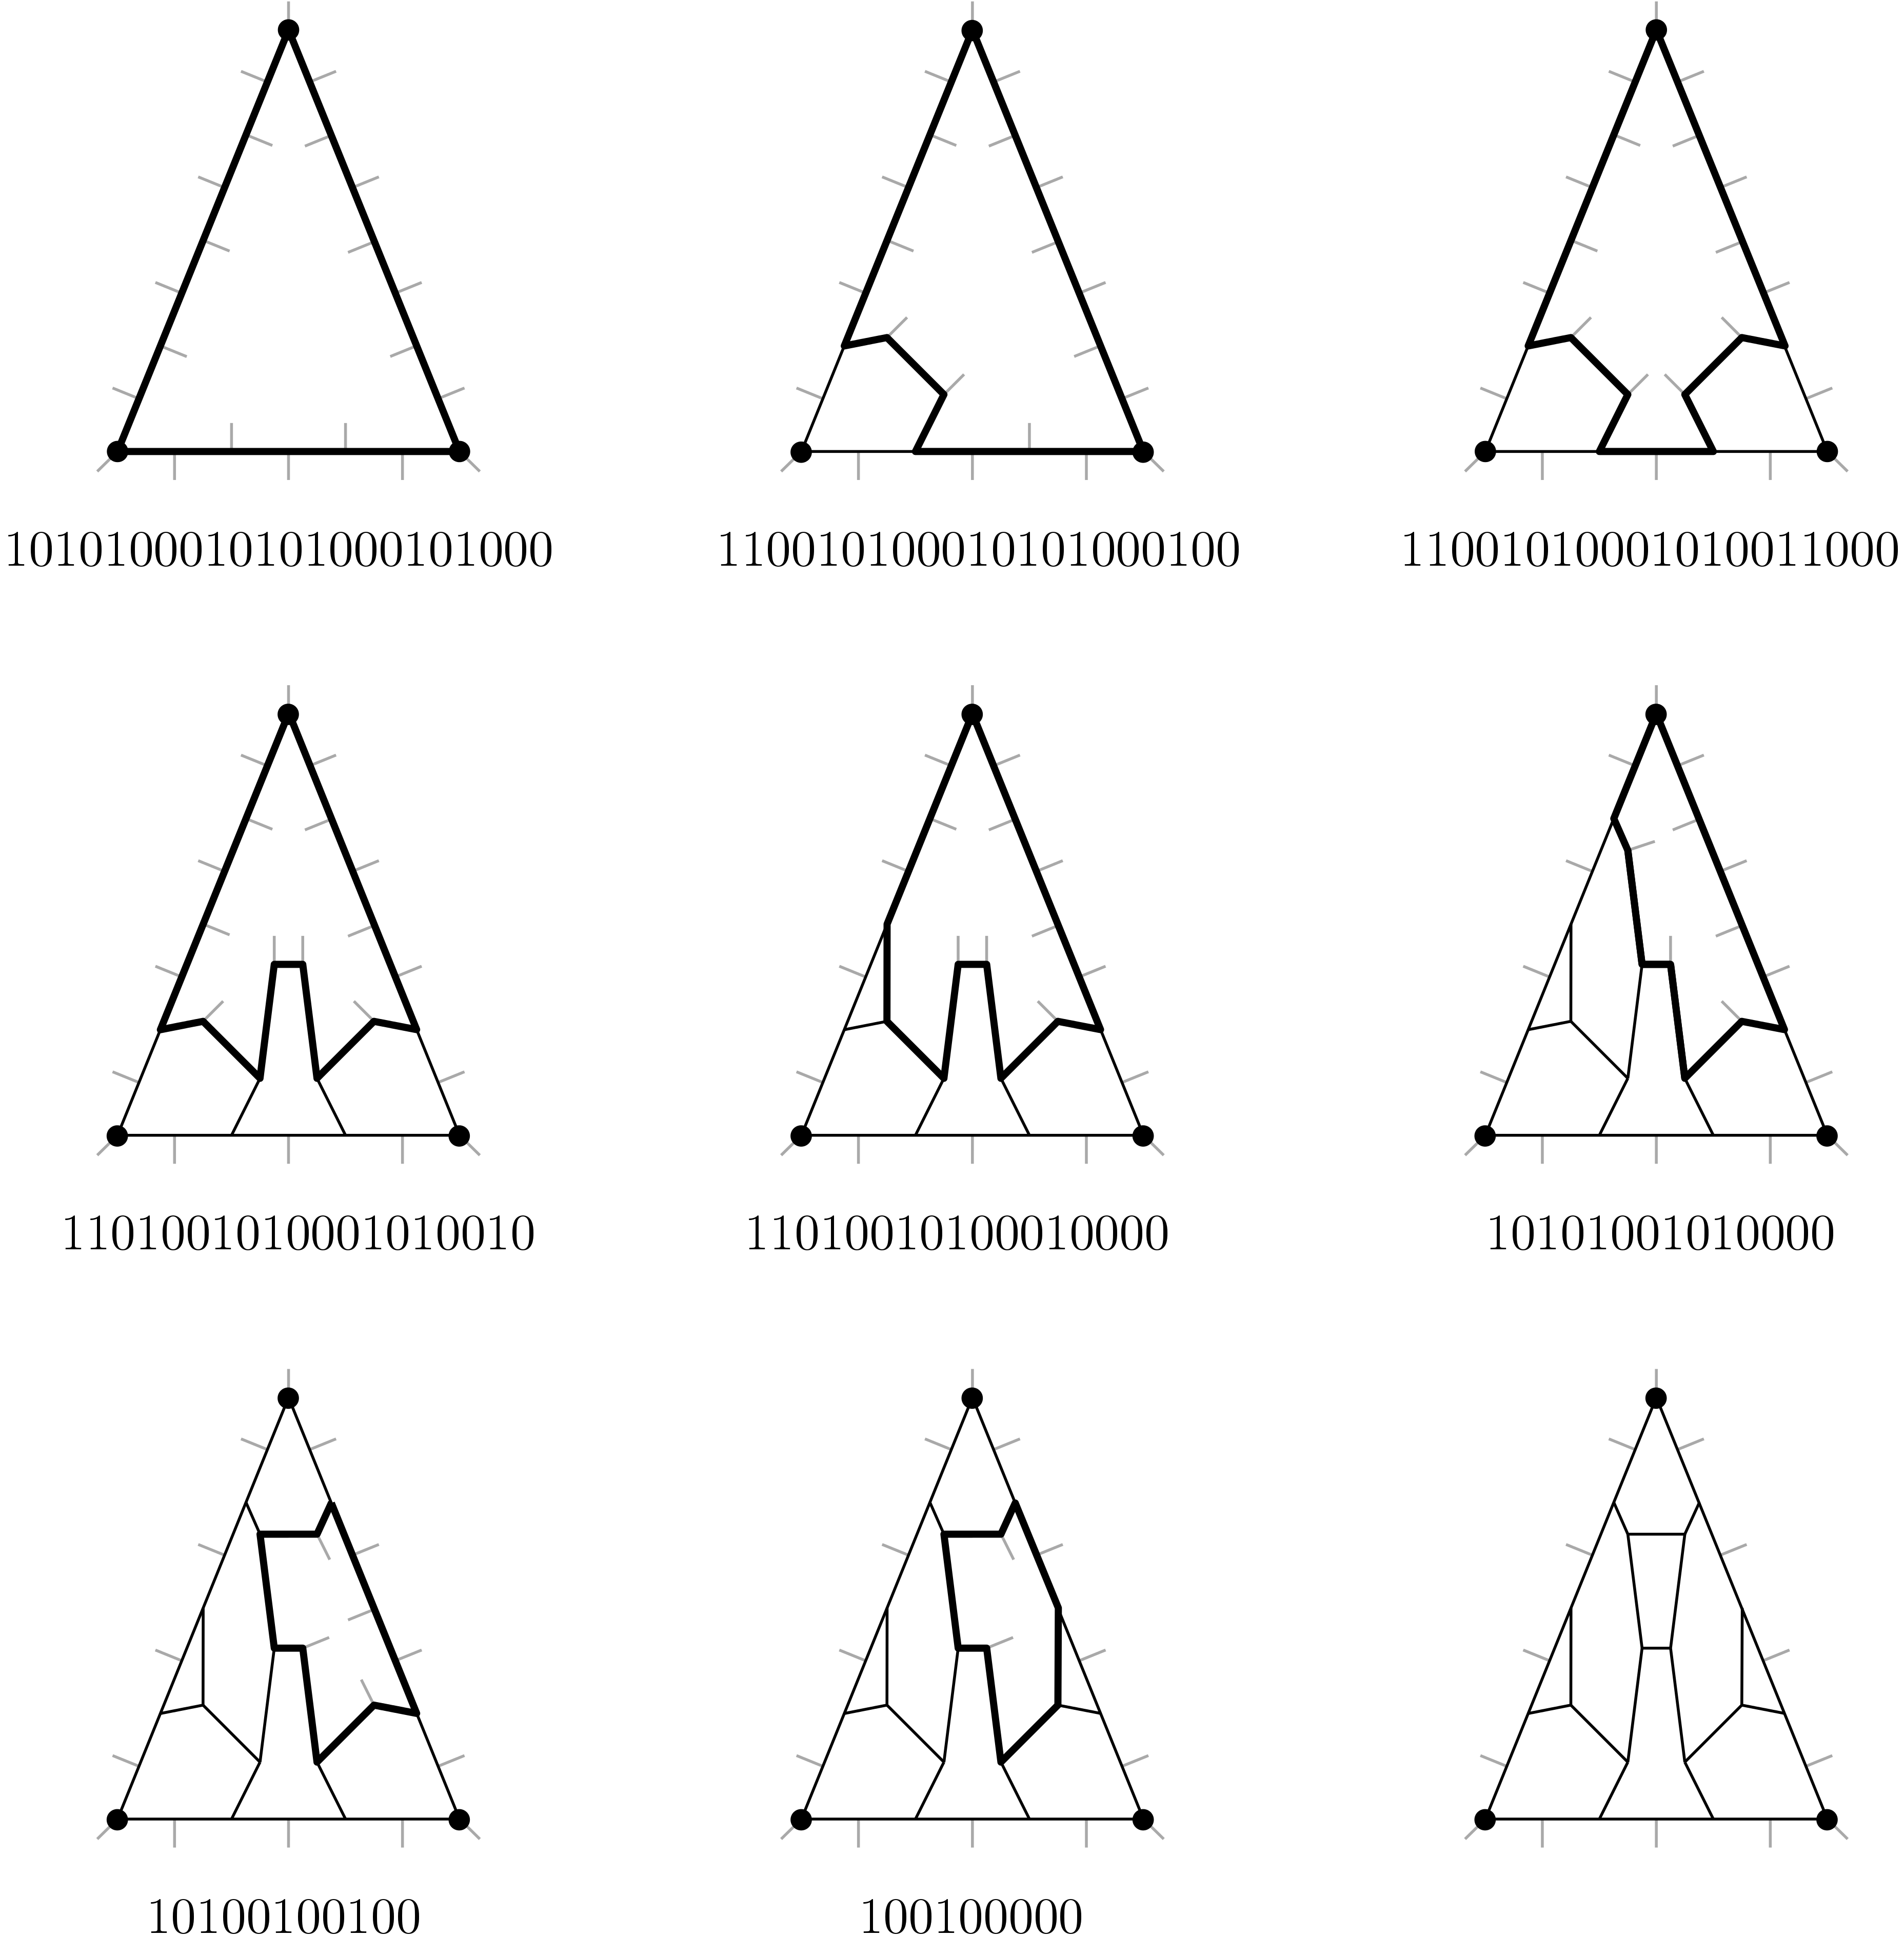
\includegraphics[width=\textwidth]{../img/reseni}
\caption{TODO popis}
\label{obr03:reseni}
\end{figure}

Pro jistotu poznamenejme, že pokud program hledaný graf nenašel, může, ale nemusí to znamenat, že neexistuje.

Podle předchozí kapitoly pro dokončení důkazu pro konkrétní dvojici $p$ a $q$ a nějaké přirozené $k$ potřebujeme tyto čtyři typy grafů:
\begin{description}
\item[(i)] ($k$, $k$, $k$),$Q$-triark;
\item[(ii)] ($k$, $k$, $k-1$),$Q$-triark;
\item[(iii)] ($mk$,$mk$,$x$),$Q\cup \lbrace 1\rbrace$-triark, kde je právě jedna stěna velikosti $l$;
\item[(iv)] prstenec, který dokáže spojit dva stejně velké, rovnostranné triarky.
\end{description}

Pro dané $k$ získáme grafy (i) a (ii) z řešítka hned. Pro zbylé je nutné pomoci si konstrukcí, která se ukázala jako úspěšná pro některé neutrální sekvence. O výsledcích získaných z programu píšeme v další kapitole. TODO odkaz?

Na graf (iii) se neumíme zeptat přímo, protože potřebujeme v grafu mít právě jednu stěnu délky $p_l$. Spojme proto stěnu s vnější stěnou triarku ručně a ptejme se na výplň vzniklých oblastí $A$ a $B$. Ke spojení použijeme $l$ kopií řetízku $R$, každý napojíme na jeden z vrcholů jádra a druhé konce spojíme s \uv{in} vrcholy základny triarku. V řetízku navíc fixujeme, ve které straně od něj budou mít které jeho vrcholy třetího souseda (znázorněno šedě v obrázku TODO odkaz). Konstrukce je obecná pro všechny přípustné hodnoty $l$, tedy není závislá na volbě $p$. Navíc není (při dobré volně R) vynucená ani příliš velká stěna, takže konstrukce může být obecná i pro všechny q (protože q je neutrální, tedy v ní musí být nenulová hodnota na pozici reprezentující stěnu velikosti alespoň 6, tvrzení \eqref{veta:posloupnosti}.



Podobnou konstrukci tvoříme i pro graf typu (iv). V tomto případě za pomoci řetízků spojujeme odpovídající vrcholy rovnostranných, stejně velkých triarků $T_1$ a $T_2$. Vzniknou dva typy oblastí - $C$ při rozích triarku a $D$ mezi odpovídajícími kusy stran triarků. Poznamenejme, že na obrázku je $T_2$ nakreslen "naruby" TODO lepší slovo?. 

Tyto konstrukce jsou v řešítku implementovány. Výsledný program tedy na vstupu očekává seznam velikostí stěn, které mohou tvořit neutrální posloupnost. Pokud pro daný seznam stěn existuje více neutrálních posloupností, využije program pro každý pomocný graf libovolnou z nich.

\begin{figure}[h!]\centering
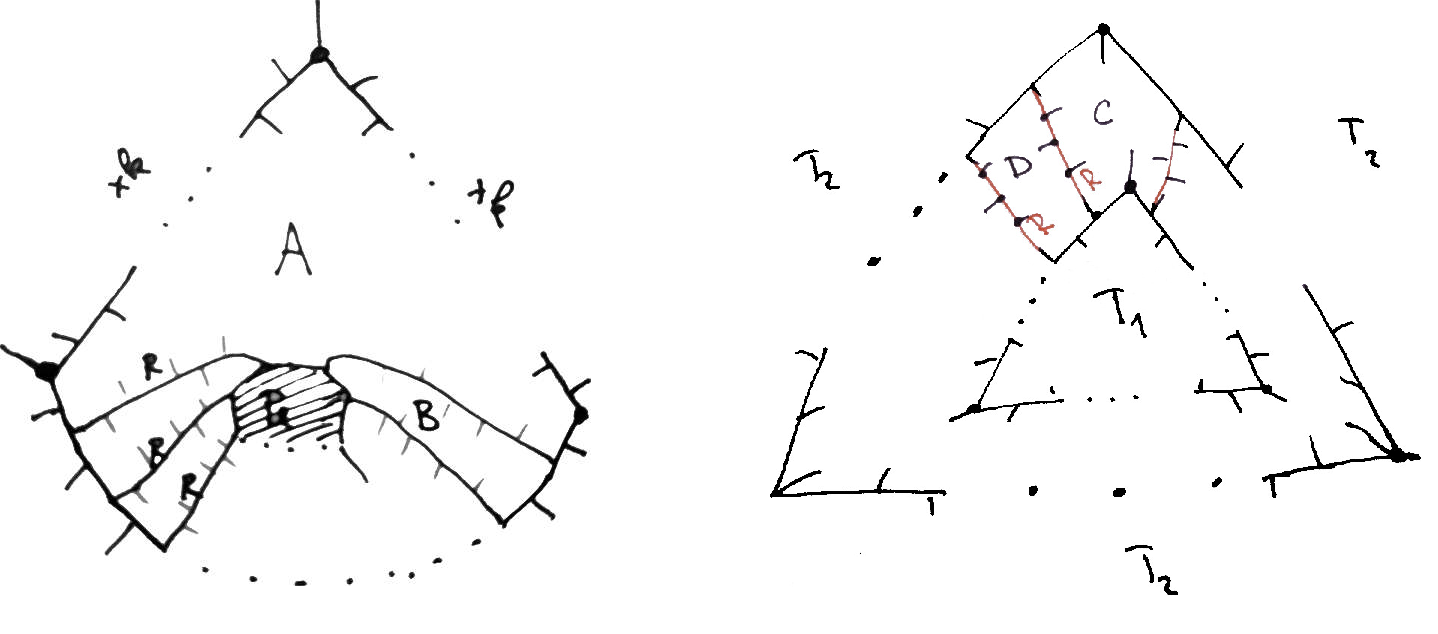
\includegraphics[height=120mm]{../img/iii+iv-construction}
\caption{Vlevo konstrukce grafu typu (iii), konkrétně ($xk$,$xk$,$l+1$)-triarku s jádrem velikosti $l$, vpravo konstrukce grafu typu (iv).}
\label{obr03:konstrukce}

\end{figure}

\section{Uživatelská dokumentace}



%%% Fiktivní kapitola s instrukcemi k PDF/A

\chapter{Výsledky} \label{vysledky}

Díky programu popsanému v předchozí kapitole bylo možné zkusit dokončit důkaz věty \eqref{veta02:hypoteza} pro některé neutrální posloupnosti $q$ (na volbě posloupnosti $p$ nezáleží, protože konstrukce pro jádrový triark nezávisí na velikosti jádra). 

Vzhledem k výpočetním omezením programu jsme zkusili dokončit důkaz věty pouze pro takové neutrální posloupnosti $q$, že $Q = {r, s}$ a navíc $r<s<18$. Seznam posloupností, pro které program nalezl potřebné grafy je v tabulce \ref{obr03:tabvysledky}. Pokud bychom se omezili na rozsah $r<s<14$, pak program grafy nalezl právě tehdy, když $r$ a $s$ jsou nesoudělná čísla.

\begin{figure}[h]\centering
\begin{tabular}{ c c c c c c c c c c c c }
  - & 7 & 8 & 9 & 10 & 11 & 12 & 13 & 14 & 15 & 16 & 17 \\
  3 & $\bullet$ & $\bullet$ &  & $\bullet$ & $\bullet$ &  & $\bullet$ & $\bullet$ &  & $\bullet$ & $\bullet$ \\
  4 & $\bullet$ &  & $\bullet$ &  & $\bullet$ &  & $\bullet$ &  & $\bullet$ \\
  5 & $\bullet$ & $\bullet$ & $\bullet$ &  & $\bullet$ & $\bullet$ & $\bullet$  
\end{tabular}
\caption{Úplný výčet dvojic stran, pro které se podařilo dokončit důkaz věty \eqref{veta02:hypoteza}.}
\label{obr03:tabvysledky}
\end{figure}
TODO označneí

Všechny potřebné grafy pro doložení důkazu jsou k práci přiloženy. TODO přiložit

Přirozenou snahou při zkoumání nalezených grafů je grafy zobrazit, aby byly pro člověka dobře čitelné. V další sekci se tomuto tématu krátce věnujeme. 

\section{Kreslení}

Přirozenou snahou pro studování nalezených grafů, a pochopení, proč právě soudělnost velikosti stěn zabraňuje v použití navrženého algoritmu k dokončení důkazu, je jejich zobrazení, které je pro člověka dostatečně čitelné. Překvapivě, i přes rovinnost grafů a celkem dobré znalosti jejich struktury není jednoduché hezké rovinné nakreslení najít.

Zamysleme se, jak graf bude vypadat. Vrcholy vnější stěny rozmístěme po kružnici a pak - podle jednotlivých hranic, které graf řeší - vždy vrcholy nově uzavřené stěny nakresleme na soustřednou, menší kružnici tak, aby spojnice žádného bodu hranice se středem kružnic neprotínala jiný bod hranice. Tímto způsobem určitě získáme rovinné nakreslení (ale hrany mohou být libovolné křivky), protože v každém kroku je možné spojit libovolné dva vrcholy, které mohou být v řešení zrovna spojovány, tak, abychom zachovali požadovanou vlastnost tvaru hranice.

Problémem takového nakreslení je počet soustředných kružnic, které bychom potřebovali, který odpovídá počtu stěn grafu. Množství potřebných kružnic by šlo celkem jednoduše snížit. Nově přidávané vrcholy nakreslíme vždy na největší kružnici, na které v příslušné výseči ještě žádný vrchol neleží. Dalším problémem by bylo rozložení vrcholů do výsečí. Představme si třeba zadání, ve kterém značný podíl tvoří souvislá posloupnost \uv{out} vrcholů. Pokud ve výpočtu dojde k uzavření stěny, která tyto vrcholy obsahuje, až na závěr, bude výseč, ve které leží, jinak zcela prázdná.

Další možností jsou běžně dostupné programy či funkce na kreslení grafů. Posouzení jejich kvality na náhodném z malých nalezených grafů necháváme na čtenáři.

Nejuspokojivější nalezenou možností je Tuttův (barycentrický) algoritmus. Jak název napovídá, jde o umisťování vrcholů do \uv{těžišť}. Nejprve je třeba rozdělit vrcholy do dvou skupin: pevné a volné. Pevné vrcholy jsou rozestaveny, aby tvořily konvexní n-úhelník. Pozice volných vrcholů se pak dopočítá jako vážený průměr sousedních vrcholů, tedy stačí řešit soustavu lineárních rovnic.

Aby mohl algoritmus dobře fungovat, je nutné, aby graf byl 3-souvislý (že jde i o postačující podmínku ukazuje článek  \cite{Tutte}). Pokud by nebyl 3-souvislý, pak vrcholy komponenty, která by po odebrání dvou vrcholů byla oddělena od zbytku grafu a neobsahovala by pevné vrcholy, budou ležet v jedné přímce.

Pro převedení grafu na 3-souvislý stačí do každé vnitřní stěny vložit nový vrchol a spojit ho se všemi vrcholy dané stěny. Ze způsobu, kterým graf vzniká, víme, že je 2-souvislý. Uvažujme nyní situaci po odebrání dvou vrcholů, které způsobí rozpadnutí grafu na více komponent. V každé nově vzniklé komponentě je vrchol, který je nově ve \uv{vnější stěně} a před odebráním byl ve stěně, ve které je i jiný vrchol než $u$ a $v$. To znamená, že po přidání vrcholů pro stěny bude jedním z nich spojen s další komponentou a tedy bude 3-souvislý. 

V našem případě za pevné vrcholy volíme vrcholy vnější stěny, které jsou rozmístěné na kružnici a podle konkrétního grafu je pak možné nastavit váhy jednotlivých vrcholů. Obecně se pro dostatečně malé grafy (do 40-ti vrcholů) osvědčila lineární závislost váhy na pořadí přidání vrcholu do grafu, nejdříve přidaný je nejtěžší.



\begin{figure}[h]\centering
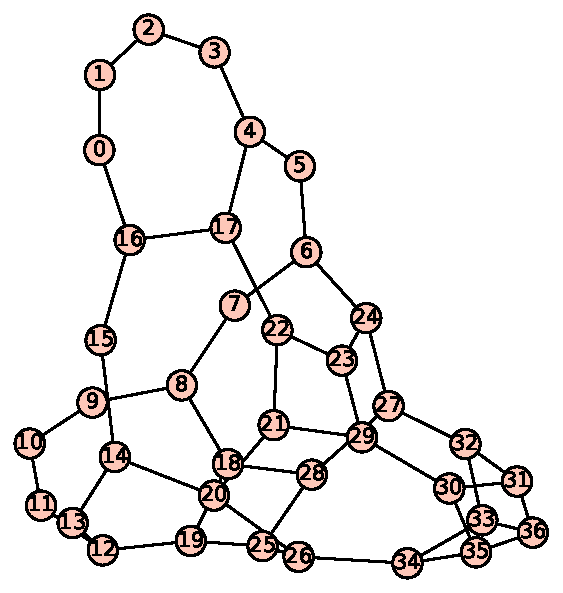
\includegraphics[width = 60mm]{../img/sageplot}
\caption{Automatické nakreslení SageMath.}
\label{obr:sageplot}
\end{figure}


\begin{figure}[h]\centering
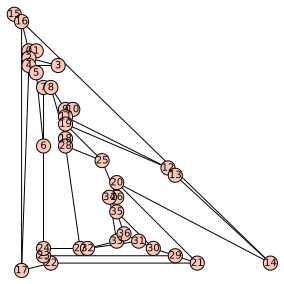
\includegraphics[width = 60mm]{../img/planar}
\caption{Rovinné nakreslení SageMath.}
\label{obr:planar}
\end{figure}


\begin{figure}[h]\centering
\includegraphics[width = 60mm]{../img/Triarc15150{4,7}__v37}
\caption{Neato s předdefinovanými pozicemi vnější stěny.}
\label{obr:Triarc15150{4,7}__v37}
\end{figure}


\begin{figure}[h]\centering
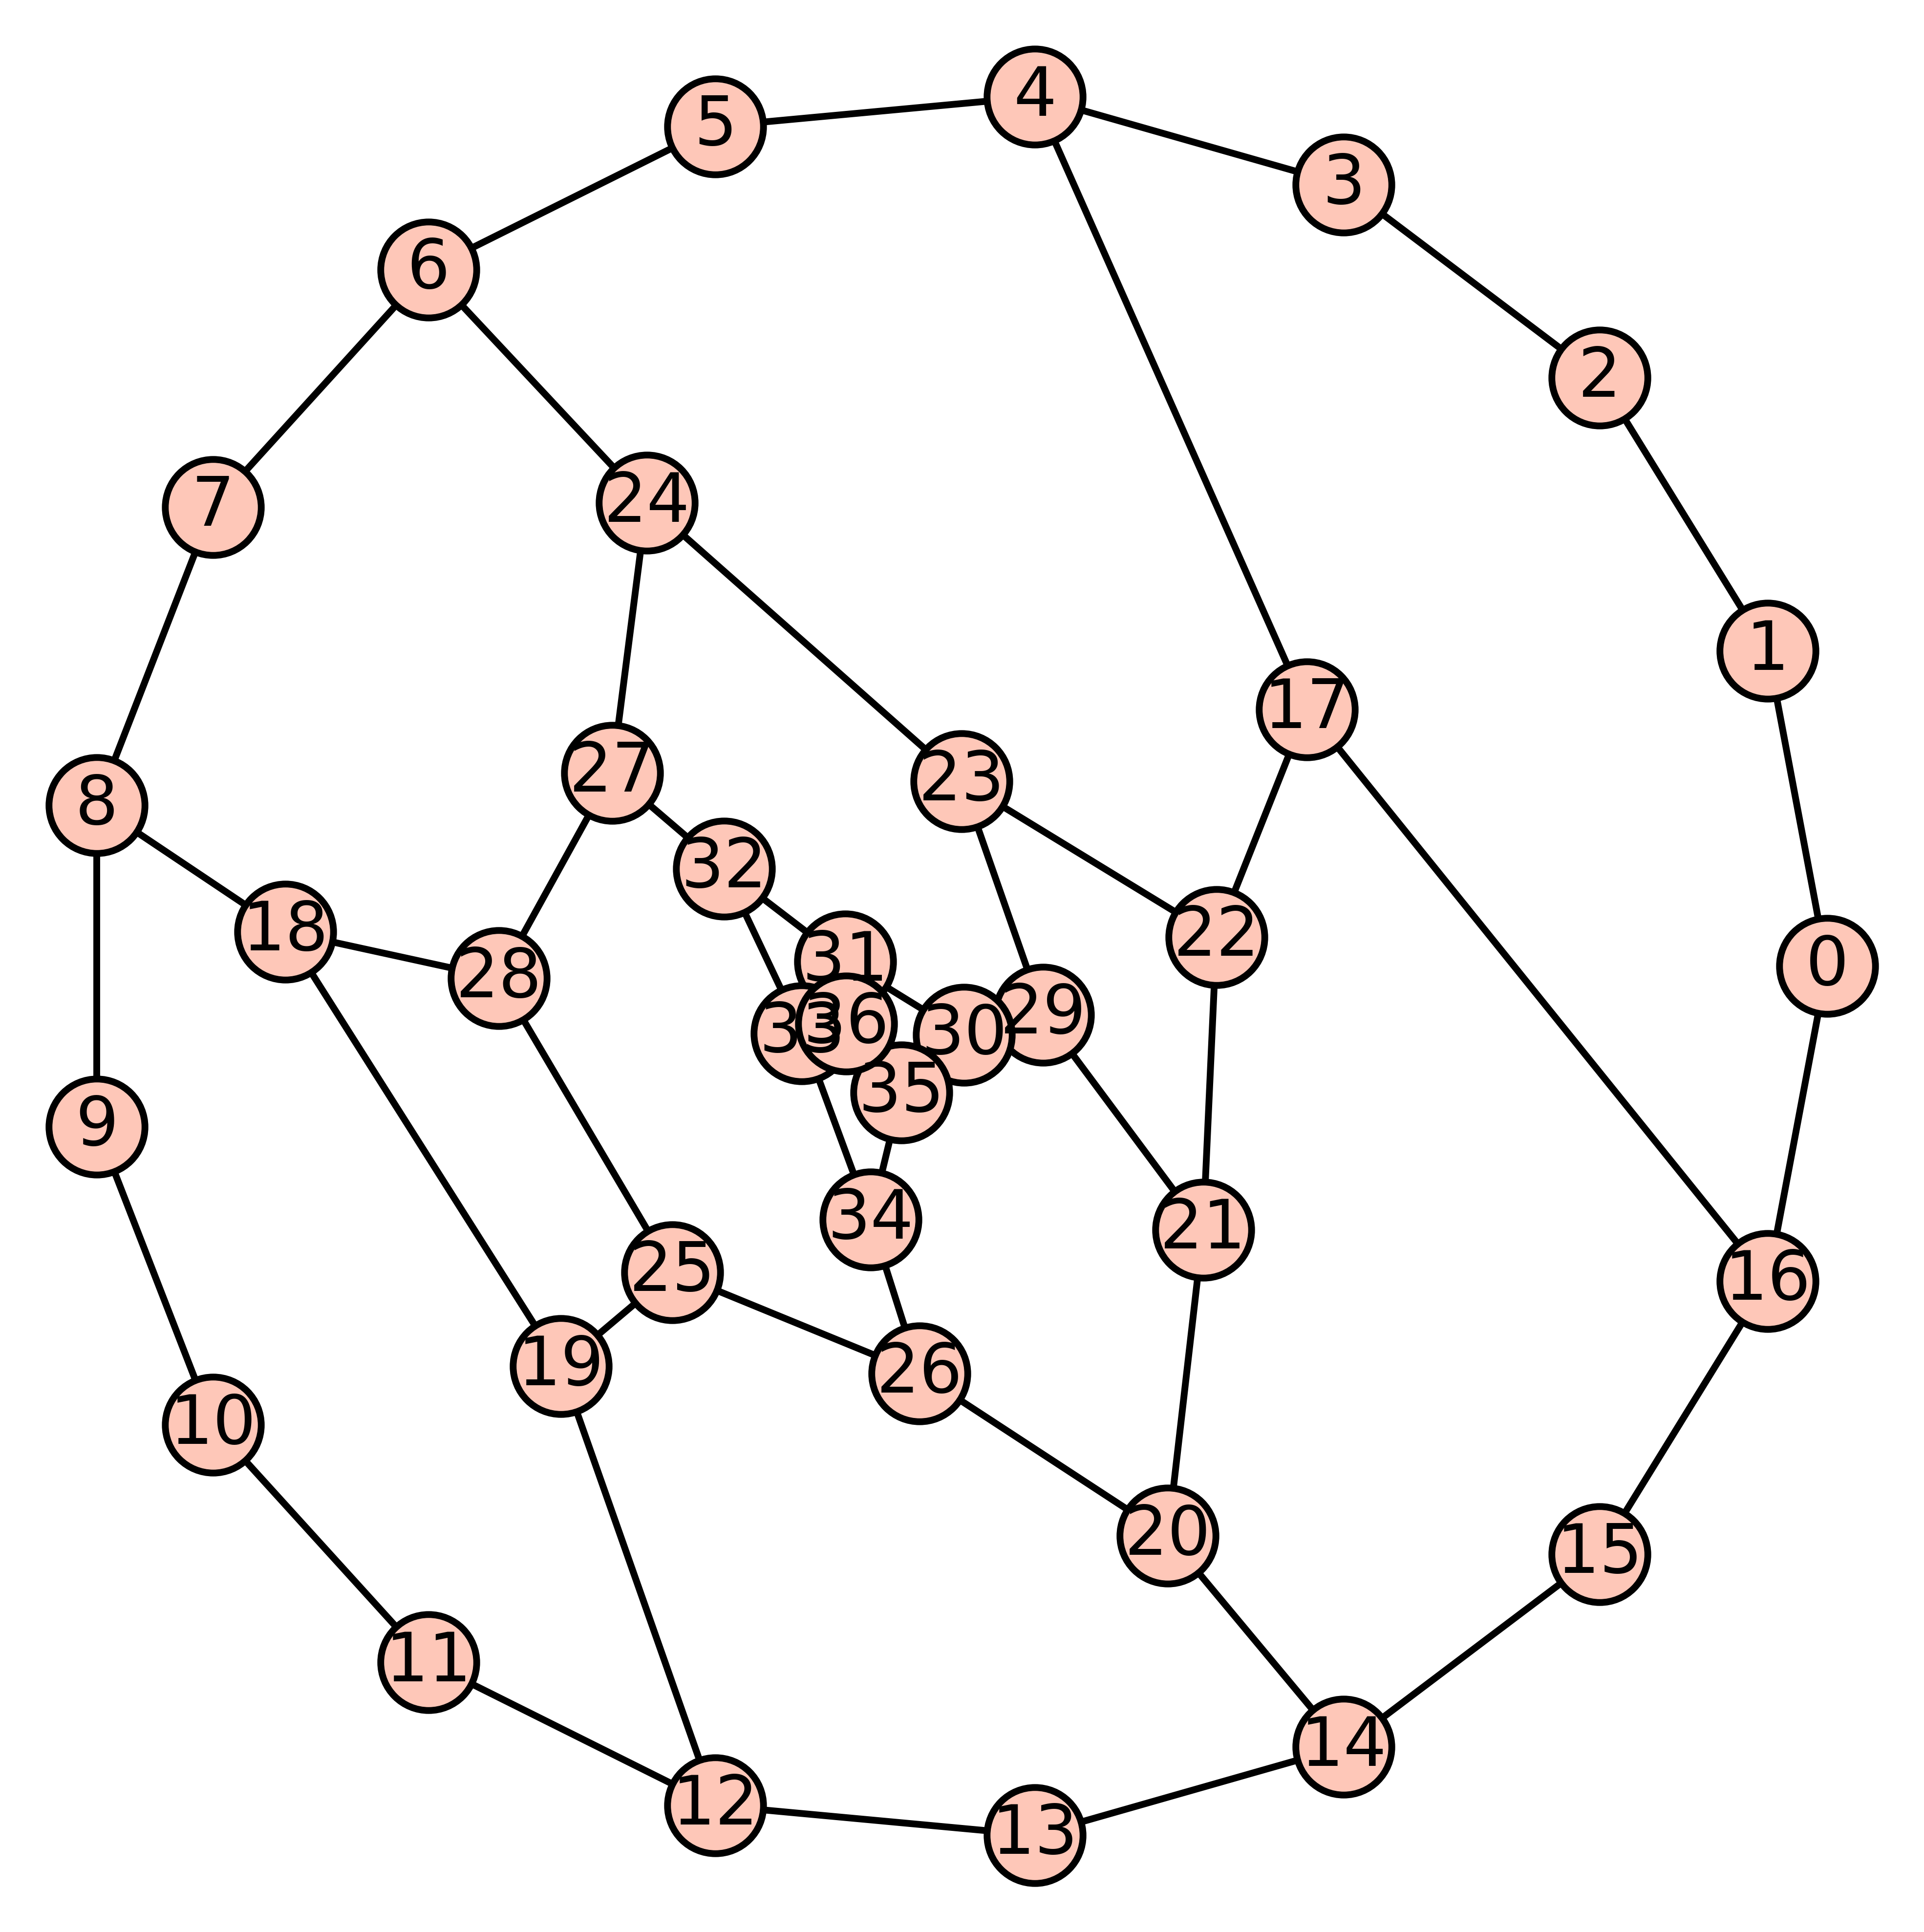
\includegraphics[width = 60mm]{../img/tutteplot}
\caption{Tuttovo nakreslení.}
\label{obr:tutteplot}
\end{figure}



\chapter{Výsledky} \label{vysledky}

Díky programu popsanému v předchozí kapitole bylo možné zkusit dokončit důkaz Věty \ref{veta02:hypoteza} pro některé neutrální posloupnosti $q$ (na volbě posloupnosti $p$ nezáleží, protože konstrukce pro jádrový triark nezávisí na velikosti jádra). 

Vzhledem k výpočetním omezením programu jsme zkusili dokončit důkaz věty pouze pro takové neutrální posloupnosti $q$, že $Q = \lbrace r, s\rbrace$ a navíc $r<s<18$. Seznam posloupností, pro které program nalezl potřebné grafy je v Tabulce \ref{obr03:tabvysledky}. Pokud bychom se omezili na rozsah $r<s<14$, pak program grafy nalezl právě tehdy, když $r$ a $s$ jsou nesoudělná čísla.

\begin{table}[h]\centering
\begin{tabular}{ c | c c c c c c c c c c c }
  {$r\setminus s$} & 7 & 8 & 9 & 10 & 11 & 12 & 13 & 14 & 15 & 16 & 17 \\ \hline
  3 & $\bullet$ & $\bullet$ &  & $\bullet$ & $\bullet$ &  & $\bullet$ & $\bullet$ &  & $\bullet$ & $\bullet$ \\
  4 & $\bullet$ &  & $\bullet$ &  & $\bullet$ &  & $\bullet$ &  & $\bullet$ \\
  5 & $\bullet$ & $\bullet$ & $\bullet$ &  & $\bullet$ & $\bullet$ & $\bullet$  
\end{tabular}
\caption{Úplný výčet dvojic stran, pro které se podařilo dokončit důkaz Věty~\ref{veta02:hypoteza}.}
\label{obr03:tabvysledky}
\end{table}

Formulujme výsledek do věty.

\begin{veta} \label{veta:vysledek}
Pro každou neutrální posloupnost $q$, která má nenulové hodnoty pouze pro $q_r$ a $q_s$, kde $r,s$ je vyznačená dvojice z Tabulky \ref{obr03:tabvysledky}, platí následující: 
mějme přípustnou posloupnost $p=(p_k | 3 \leq k \neq 6)$, pak existuje nekonečně takových přirozených $n$, že $p+nq$ je realizovatelná.
\end{veta}


\begin{table}[h]\centering
\resizebox{0.7\textwidth}{!}{%
\begin{tabular}{| c || c | c | c |}

\hline 
{$s\setminus r$} & 3 &4&5 \\ \hline \hline

7 & \cellcolor{lightgray}(i): 3 & \cellcolor{lightgray}(i): 3 & \cellcolor{lightgray}(i): 3\\
 & \cellcolor{lightgray}(ii): 3 & \cellcolor{lightgray}(ii): 3 & \cellcolor{lightgray}(ii): 3\\
 & \cellcolor{lightgray}AB : 101010 & \cellcolor{lightgray}AB : 101010 & \cellcolor{lightgray}AB : 101010\\
 & \cellcolor{lightgray}CD : 101010 & \cellcolor{lightgray}CD : 101010 & \cellcolor{lightgray}CD : 1010\\\hline

8 & \cellcolor{lightgray}(i): 3 & (i): 3,5,6,9 & \cellcolor{lightgray}(i): 3\\
 & \cellcolor{lightgray}(ii): 3 & (ii):  & \cellcolor{lightgray}(ii): 3\\
 & \cellcolor{lightgray}AB : 1010 & AB :  & \cellcolor{lightgray}AB : 1010\\
 & \cellcolor{lightgray}CD : 1010 & CD :  & \cellcolor{lightgray}CD : 1010\\\hline

9 & (i): 3,4,8 & \cellcolor{lightgray}(i): 3 & \cellcolor{lightgray}(i): 3\\
 & (ii):  & \cellcolor{lightgray}(ii): 3 & \cellcolor{lightgray}(ii): 3\\
 & AB :  & \cellcolor{lightgray}AB : 1010 & \cellcolor{lightgray}AB : 1010\\
 & CD :  & \cellcolor{lightgray}CD : 1010 & \cellcolor{lightgray}CD : 1010\\\hline

10 & \cellcolor{lightgray}(i): 3 & (i): 3,4,5,6,7,8,9,10 & (i): 4,5,9,10\\
 & \cellcolor{lightgray}(ii): 3 & (ii):  & (ii): \\
 & \cellcolor{lightgray}AB : 1010 & AB :  & AB : \\
 & \cellcolor{lightgray}CD : 1010 & CD : 1010 & CD : \\\hline

11 & \cellcolor{lightgray}(i): 3 & \cellcolor{lightgray}(i): 3 & \cellcolor{lightgray}(i): 3\\
 & \cellcolor{lightgray}(ii): 3 & \cellcolor{lightgray}(ii): 3 & \cellcolor{lightgray}(ii): 3\\
 & \cellcolor{lightgray}AB : 1010 & \cellcolor{lightgray}AB : 1010 & \cellcolor{lightgray}AB : 1010\\
 & \cellcolor{lightgray}CD : 1010 & \cellcolor{lightgray}CD : 1010 & \cellcolor{lightgray}CD : 1010\\\hline

12 & (i): 3,4,5,6,7,8,9,10 & (i): 5,6 & \cellcolor{lightgray}(i): 3\\
 & (ii):  & (ii):  & \cellcolor{lightgray}(ii): 3\\
 & AB :  & AB :  & \cellcolor{lightgray}AB : 1010\\
 & CD :  & CD :  & \cellcolor{lightgray}CD : 1010\\\hline

13 & \cellcolor{lightgray}(i): 3 & \cellcolor{lightgray}(i): 3 & \cellcolor{lightgray}(i): 3\\
 & \cellcolor{lightgray}(ii): 3 & \cellcolor{lightgray}(ii): 3 & \cellcolor{lightgray}(ii): 3\\
 & \cellcolor{lightgray}AB : 1010 & \cellcolor{lightgray}AB : 1010 & \cellcolor{lightgray}AB : 1010\\
 & \cellcolor{lightgray}CD : 1010 & \cellcolor{lightgray}CD : 1010 & \cellcolor{lightgray}CD : 1010\\\hline

14 & \cellcolor{lightgray}(i): 3 & (i): 3,4,5,6,7,8,9,10 & (i): \\
 & \cellcolor{lightgray}(ii): 3 & (ii):  & (ii): \\
 & \cellcolor{lightgray}AB : 1010 & AB :  & AB : \\
 & \cellcolor{lightgray}CD : 1010 & CD : 1010 & CD : \\\hline

15 & (i): 3,4,7,8 & \cellcolor{lightgray}(i): 3 & (i): 9,10\\
 & (ii):  & \cellcolor{lightgray}(ii): 3 & (ii): \\
 & AB :  & \cellcolor{lightgray}AB : 1010 & AB : \\
 & CD :  & \cellcolor{lightgray}CD : 1010 & CD : \\\hline

16 & \cellcolor{lightgray}(i): 3 & (i): 3,5,6,8,9 & (i): \\
 & \cellcolor{lightgray}(ii): 3 & (ii):  & (ii): \\
 & \cellcolor{lightgray}AB : 1010 & AB :  & AB : \\
 & \cellcolor{lightgray}CD : 1010 & CD :  & CD : \\\hline

17 & \cellcolor{lightgray}(i): 3 & (i):  & (i): \\
 & \cellcolor{lightgray}(ii): 3 & (ii):  & (ii): \\
 & \cellcolor{lightgray}AB : 1010 & AB :  & AB : \\
 & \cellcolor{lightgray}CD : 1010 & CD :  & CD : \\\hline

\end{tabular}}
\caption{Přehled nalezených grafů. Ohraničené buňky kódují výsledek pro danou dvojici $r$, $s$. Pokud jsou grafy nalezené, je buňka šedá. První řádek buňky: $k$ pro nalezené ($k$, $k$, $k$)-triarky; druhý: $k$ pro nalezené ($k$, $k$, $k$)- a zároveň ($k$, $k$, $k-1$)-triarky; třetí: řetízek pro konstrukci grafu (iii), kde $mk$ odpovídá poslední hodnotě v druhém řádku; čtvrtý: řetízek pro graf (iv).}
\label{obr03:tabvysledkycele}
\end{table}

Všechny potřebné grafy pro doložení důkazu jsou v Příloze \ref{priloha:vysledky}.

\chapter*{Závěr}
\addcontentsline{toc}{chapter}{Závěr}


%%% Seznam použité literatury
%%% Seznam použité literatury (bibliografie)
%%%
%%% Pro vytváření bibliografie používáme bibTeX. Ten zpracovává
%%% citace v textu (např. makro \cite{...}) a vyhledává k nim literaturu
%%% v souboru literatura.bib.
%%%
%%% Příkaz \bibliographystyle určuje, jakým stylem budou citovány odkazy
%%% v textu. V závorce je název zvoleného souboru .bst. Styly plainnat
%%% a unsrt jsou standardní součástí latexových distribucí. Styl czplainnat
%%% je dodáván s touto šablonou a bibTeX ho hledá v aktuálním adresáři.

\bibliographystyle{czplainnat}    %% Autor (rok) s českými spojkami
% \bibliographystyle{plainnat}    %% Autor (rok) s anglickými spojkami
% \bibliographystyle{unsrt}       %% [číslo]

\renewcommand{\bibname}{Seznam použité literatury}

%%% Vytvoření seznamu literatury. Pozor, pokud jste necitovali ani jednu
%%% položku, seznam se automaticky vynechá.

\bibliography{literatura}

%%% Kdybyste chtěli bibliografii vytvářet ručně (bez bibTeXu), lze to udělat
%%% následovně. V takovém případě se řiďte normou ISO 690 a zvyklostmi v oboru.

% \begin{thebibliography}{99}
%
% \bibitem{lamport94}
%   {\sc Lamport,} Leslie.
%   \emph{\LaTeX: A Document Preparation System}.
%   2. vydání.
%   Massachusetts: Addison Wesley, 1994.
%   ISBN 0-201-52983-1.
%
% \end{thebibliography}


%%% Obrázky v bakalářské práci
%%% (pokud jich je malé množství, obvykle není třeba seznam uvádět)
\listoffigures

%%% Tabulky v bakalářské práci (opět nemusí být nutné uvádět)
%%% U matematických prací může být lepší přemístit seznam tabulek na začátek práce.
%\listoftables

%%% Použité zkratky v bakalářské práci (opět nemusí být nutné uvádět)
%%% U matematických prací může být lepší přemístit seznam zkratek na začátek práce.
%\chapwithtoc{Seznam použitých zkratek}

%%% Přílohy k bakalářské práci, existují-li. Každá příloha musí být alespoň jednou
%%% odkazována z vlastního textu práce. Přílohy se číslují.
%%%
%%% Do tištěné verze se spíše hodí přílohy, které lze číst a prohlížet (dodatečné
%%% tabulky a grafy, různé textové doplňky, ukázky výstupů z počítačových programů,
%%% apod.). Do elektronické verze se hodí přílohy, které budou spíše používány
%%% v elektronické podobě než čteny (zdrojové kódy programů, datové soubory,
%%% interaktivní grafy apod.). Elektronické přílohy se nahrávají do SISu a lze
%%% je také do práce vložit na CD/DVD. Povolené formáty souborů specifikuje
%%% opatření rektora č. 72/2017.
\appendix
\chapter{Přílohy}
Přiložený disk obsahuje zdrojové kódy aplikace, spustitelnou aplikaci a výsledky, které jsme získali.

\section{Aplikace}
Přikládáme zdrojové kódy v \texttt{C\#} (.NET Framework 4.6.1) v podobě kompletního projektu pro  Visual Studio 2015. A také zkompilovaný program, který zpřístupňuje uživatelům Windows aplikaci bez nutné instalace.
 
\section{Získané výsledky} \label{priloha:vysledky}
Přikládáme grafy, které dokazují pravdivost hlavního výsledku, Věty \ref{veta:vysledek}. Pro každou dvojici stěn $r$, $s$, která je v Tabulce~\ref{obr03:tabvysledky} označena, je ve složce \texttt{grafy} přiložena složka s velikostmi stěn v názvu. V ní jsou shrnuté parametry nalezených grafů a podadresáře s jednotlivými grafy, ve všech formátech popsaných v Sekci \ref{prg&vystupy}.
\openright
\end{document}
